\documentclass[11pt]{article}
\usepackage{calc}
\usepackage[margin={1in,0.5in},footskip=0in]{geometry}
\usepackage[miniquiz]{hwk}
\usepackage{tikz, pgfplots, textcomp}

\renewcommand{\theclass}{math 1300}
\renewcommand{\dateinfo}{December 4, 2012}
\renewcommand{\theassignment}{Quiz 10}

\begin{document}
\pagestyle{empty}
\newsavebox{\quizfront}
\begin{lrbox}{\quizfront}
\begin{minipage}[top][4.5in][t]{\textwidth} \setlength{\parindent}{1.5em}
\drawtitle
\vspace{-0.5in}
\begin{enumerate}

\item A particle has the velocity function $v(t)$, given by the following graph:

\begin{center}
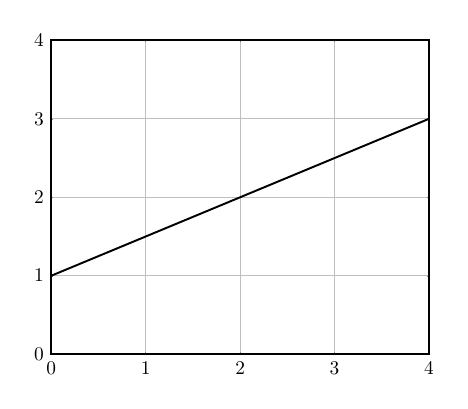
\begin{tikzpicture}[scale=0.7]
\begin{axis}[ 
	xlabel={},
	ylabel={},
	xmin=0,
	xmax=4,
	ymin=0,
	ymax=4,
	xtick={0,1,2,3,4},
	ytick={0,1,2,3,4},
	major tick length={1},
	grid=major,
	line width=1pt,] 
	\addplot [smooth] {(1/2)*x+1}; 
\end{axis}
\end{tikzpicture}
\end{center}
\vspace{-.1in}
What is the total distance travelled by the particle over the interval $t=0$ to $t=4$? 


\end{enumerate}

\vfill

\hfill\textsc{over} $\longrightarrow$


\end{minipage}
\end{lrbox}

%%%%%%%%%%%%%%%%%%%%%%%%%%%%%%%%%%%%%%%%%%%%%%%%%%%%%%
%%%% This is for the back of the quiz
%%%%%%%%%%%%%%%%%%%%%%%%%%%%%%%%%%%%%%%%%%%%%%%%%%%%%%
\newsavebox{\quizback}
\begin{lrbox}{\quizback}
\begin{minipage}[top][4.5in][t]{\textwidth} \setlength{\parindent}{1.5em}
\begin{enumerate}
\item[2.] Estimate the value of the given integral using a left
  Riemann sum with $n=4$ subdividisions:
  \[
  \int_0^4 \left( x^2 + 1 \right) \; dx.
  \]

\end{enumerate}
\end{minipage}
\end{lrbox}

%%%%%%%%%%%%%%%%%%%%%%%%%%%%%%%%%%%%%%%%%%%%%%%%%%%%%%
%%%%
%%%% Now we make two copies of the ``quizfront'' box
%%%%
%%%%%%%%%%%%%%%%%%%%%%%%%%%%%%%%%%%%%%%%%%%%%%%%%%%%%%%
\noindent \usebox{\quizfront}
\vfill
\noindent \usebox{\quizfront}

%%%% Uncomment the rest to have a two-sided quiz.
\pagebreak
\noindent \usebox{\quizback}
\vfill
\noindent \usebox{\quizback}
\end{document}